% Hlavicka pro protokoly z fyzikalniho praktika.
% Verze pro: LaTeX
% Verze hlavicky: 22. 2. 2007
% Autor: Ustav fyziky kondenzovanych latek
% Ke stazeni: www.physics.muni.cz/ufkl/Vyuka/
% Licence: volne k pouziti, nejlepe k vcasnemu odevzdani protokolu z Vaseho mereni.

\documentclass[a4paper,11pt]{article}

% Kodovani (cestiny) v dokumentu: utf-8
%\usepackage[cp1250]{inputenc}	% Omezena stredoevropska kodova stranka, pouze MSW.
\usepackage[utf8]{inputenc}	% Doporucujeme pouzivat UTF-8 (unicode).

%%% Nemente:
\usepackage[margin=2cm]{geometry}
\newtoks\jmenopraktika \newtoks\jmeno \newtoks\datum
\newtoks\obor \newtoks\skupina \newtoks\rocnik \newtoks\semestr
\newtoks\cisloulohy \newtoks\jmenoulohy
\newtoks\tlak \newtoks\teplota \newtoks\vlhkost
\usepackage{amsmath}
\usepackage{mathtools}
\usepackage{graphicx}
\usepackage{multirow}
\graphicspath{ {./images/} }
%%% Nemente - konec.


%%%%%%%%%%% Doplnte pozadovane polozky:

\jmenopraktika={Fyzikální praktikum 2}  % nahradte jmenem vaseho predmetu
\jmeno={Artem Gorodilov}            % nahradte jmenem mericiho
\datum={18. ~prosince  2023}        % nahradte datem mereni ulohy
\obor={Astrofyzika}                     % nahradte zkratkou vami studovaneho oboru
\skupina={Čt 8:00}            % nahradte dobou vyuky vasi seminarni skupiny
\rocnik={II}                  % nahradte rocnikem, ve kterem studujete
\semestr={I}                 % nahradte semestrem, ve kterem studujete

\cisloulohy={1}               % nahradte cislem merene ulohy
\jmenoulohy={Studium elektromagnetické indukce} % nahradte jmenem merene ulohy

\tlak={981}                   % nahradte tlakem pri mereni (v hPa)
\teplota={20.8}               % nahradte teplotou pri mereni (ve stupnich Celsia)
\vlhkost={43}               % nahradte vlhkosti vzduchu pri mereni (v %)

%%%%%%%%%%% Konec pozadovanych polozek.


%%%%%%%%%%% Uzitecne balicky:
\usepackage[czech]{babel}
\usepackage{graphicx}
\usepackage{amsmath}
\usepackage{xspace}
\usepackage{url}
\usepackage{indentfirst}
\usepackage{listings}
\usepackage{subcaption}
\usepackage{caption}
\usepackage{tabularx}
\usepackage{multicol}
\usepackage[labelformat=parens,labelsep=quad,skip=3pt]{caption}

%%%%%% Zamezeni parchantu:
\widowpenalty 10000 \clubpenalty 10000 \displaywidowpenalty 10000
%%%%%% Parametry pro moznost vsazeni vetsiho poctu obrazku na stranku
\setcounter{topnumber}{3}	  % max. pocet floatu nahore (specifikace t)
\setcounter{bottomnumber}{3}	  % max. pocet floatu dole (specifikace b)
\setcounter{totalnumber}{6}	  % max. pocet floatu na strance celkem
\renewcommand\topfraction{0.9}	  % max podil stranky pro floaty nahore
\renewcommand\bottomfraction{0.9} % max podil stranky pro floaty dole
\renewcommand\textfraction{0.1}	  % min podil stranky, ktery musi obsahovat text
\intextsep=8mm \textfloatsep=8mm  %\intextsep pro ulozeni [h] floatu a \textfloatsep pro [b] or [t]

% Tecky za cisly sekci:
\renewcommand{\thesection}{\arabic{section}.}
\renewcommand{\thesubsection}{\thesection\arabic{subsection}.}
% Jednopismenna mezera mezi cislem a nazvem kapitoly:
\makeatletter \def\@seccntformat#1{\csname the#1\endcsname\hspace{1ex}} \makeatother

\begin{document}

\thispagestyle{empty}

{
\begin{center}
\sf 
{\Large Ústav fyzikální elektroniky PřF MU} \\
\bigskip
{\huge \bfseries FYZIKÁLNÍ PRAKTIKUM} \\
\bigskip
{\Large \the\jmenopraktika}
\end{center}

\bigskip

\sf
\noindent
\setlength{\arrayrulewidth}{1pt}
\begin{tabular*}{\textwidth}{@{\extracolsep{\fill}} l l}
\large {\bfseries Zpracoval:}  \the\jmeno & \large  {\bfseries Naměřeno:} \the\datum\\[2mm]
\large  {\bfseries Obor:} \the\obor  \hspace{40mm}  {\bfseries Skupina:} \the\skupina %
%{\bfseries Ročník:} \the\rocnik \hspace{5mm} {\bfseries Semestr:} \the\semestr  
&\large {\bfseries Testováno:}\\
\\
\hline
\end{tabular*}
}

\bigskip

{
\sf
\noindent \begin{tabular}{p{3cm} p{0.6\textwidth}}
\Large  Úloha č. {\bfseries \the\cisloulohy:} \par
\smallskip
$T=\the\teplota$~$^\circ$C \par
$p=\the\tlak$~hPa \par
$\varphi=\the\vlhkost$~\%
&\Large \bfseries \the\jmenoulohy  \\[2mm]
\end{tabular}
}

\vskip1cm
    \begin{minipage}[t]{0.5\textwidth} 
        \section{Zadání}
            Změřit závislost tvaru napěťových impulsů na cívce na výchylce kyvadla s magnetem.
            \par Určit poloměr cívky a magnetický moment magnetu.
            \par Vyšetřit tlumení indukovaných impulzů.
        \section{Teorie}
            \subsection{Závislost indukovaných pulzů na výchylce, poloměr cívky a magnetický moment magnetu}
                Jev elektromagnetické indukce lze zkoumat pomocí systému znázorněného na obrázku (1). Tento systém se skládá z permanentního magnetu připevněného ke dvojitému kyvadlu, které kýváním indukuje napěťové impulsy v blízké cívce. Tyto impulsy jsou kvantitativně analyzovány pomocí analogově-digitálního převodníku připojeného k počítači, což umožňuje přesné měření jejich časových charakteristik.
                \par Klíčem k naší analýze je Faradayův zákon elektromagnetické indukce:
                \begin{equation}
                    U = -\frac{d\Phi}{dt}
                \end{equation}
                který popisuje, jak změny magnetického toku v obvodu způsobují elektromotorickou sílu (EMF) v cívce. Když cívkou prochází magnet, měnící se magnetické pole způsobuje kolísání indukovaného napětí. Situaci lze vidět na obrázku (2).
    \end{minipage}
    \hspace{10pt}
    \begin{minipage}[t]{0.5\textwidth} 
                \vspace{0pt}   
                \par \centering
                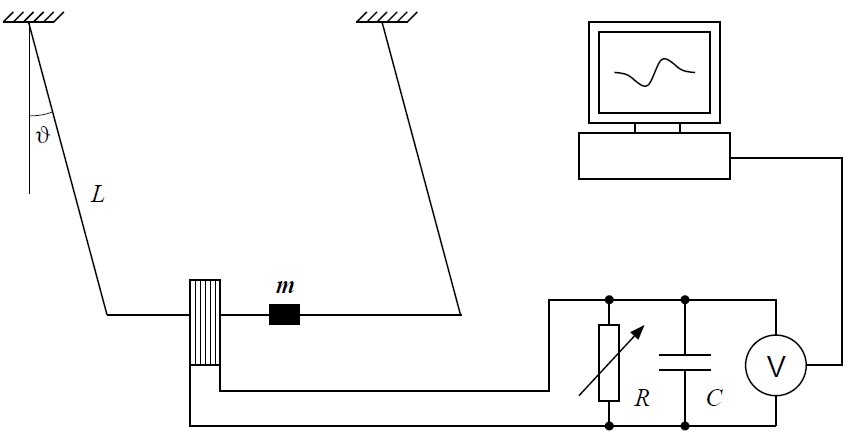
\includegraphics[scale=0.35]{scheme}
                \captionsetup{justification=centering, font=footnotesize}
                \captionof{figure}{Schéma experimentálního plánu. Permanentní magnety prolétávají cívkou, v níž se indukuje napětí, které je zaznamenáváno počítačem. Cívka je zatížena proměnným odporem o odporu $R$, který omezuje proud v obvodu, a tím přímo ovlivňuje elektromagnetický útlum pohybu magnetů. K potlačení vysokofrekvenčního šumu se používá kondenzátor s malou kapacitou $C$ (standardně 100 nF).}
                \label{fig:scheme}
                \vspace{20pt}
                \raggedright
                \par Za předpokladu konstantní rychlosti magnetu při průchodu cívkou odvodíme vztahy týkající se poloměru cívky, rychlosti magnetu a amplitudy indukovaného napětí:
                \begin{equation}
                    \Delta t = \frac{a}{\upsilon_m}
                \end{equation}
                kde $a$ je poloměr cívky. Také:
                \begin{equation}
                    \Delta t = t_{max} - t_{min}
                \end{equation}
                kde $t_min$ je minimální čas a $t_max$ je maximální čas. 
    \end{minipage}
\newpage
                \begin{figure}[ht!]
                    \centering
                    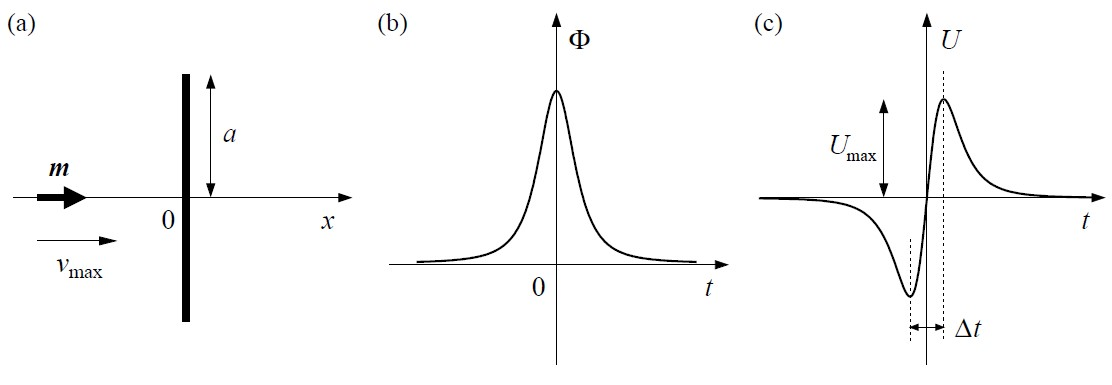
\includegraphics[scale=0.55]{imp}
                    \captionsetup{justification=centering, font=footnotesize}
                    \captionof{figure}{(a) Boční pohled na kruhovou cívku o poloměru $a$, kterou prochází magnet s dipólovým momentem $m$. (b) Závislost magnetického a proudu na čase. (c) Napětí indukované v kruhovém závitu.}
                    \label{fig:imp}
                \end{figure}
    \begin{minipage}[t]{0.5\textwidth} 
                \begin{equation}
                    \upsilon_m = 2\sqrt{gL} ~sin\left(\frac{\vartheta_{max}}{2}\right) \approx \sqrt{gL} ~\vartheta_{max}
                \end{equation}
                kde $g$ je místní zrychlení volného pádu, $L$ je délka kyvadla a $\vartheta_{max}$ je amplituda výchylky kmitů.  
                \par V tomto případě je amplituda napěťových impulsů $U_{max}$ přímo úměrná úhlu vychýlení kmitání. 
                \begin{equation}
                    U_{max} = \frac{U - U_{min}}{2}
                \end{equation}
                kde $U_{min}$ je minimální napětí a $U$ je maximální napětí. 
                \begin{equation}
                    U_{max} = k\vartheta_{max}
                \end{equation}
                kde $k$ je koeficient úměrnosti.
                \par Magnetický dipólový moment $m$ lze určit na základě znalosti koeficientu úměrnosti $k$ a poloměru cívky $a$:
                \begin{equation}
                    m = \frac{25\sqrt{5}}{24} \frac{k a^2}{\mu_0 N \sqrt{gL}}
                \end{equation}
                kde $N$ je počet závitů cívky a $\mu_0$ je permeabilita vakua. 
            \subsection{Tlumení indukovaných pulzů}
                Dále zkoumáme účinky tlumení indukovaných impulzů. Tyto účinky vznikají jak mechanicky, zejména v důsledku odporu vzduchu, tak elektromagneticky. 
                K určení mechanického koeficientu tlumení $\beta$ můžeme použít následující vzorec: 
                \begin{equation}
                    U_M(t) = U_{M,0}e^{-\beta t}
                \end{equation}
                kde $U_{M,0}$ je počáteční napětí při daném odporu a $U_M(t)$ je napětí v čase $t$.
                \par Pro určení elektromagnetického útlumu $\alpha$ můžeme použít vzorec: 
    \end{minipage}
    \hspace{10pt}
    \begin{minipage}[t]{0.5\textwidth}
                \begin{equation}
                    U_{M}(t) = U_{M, 0} - \alpha t
                \end{equation}
                kde $U_{M, 0}$ je počáteční amplituda při daném odporu a $U_{M}(t)$ je amplituda v čase $t$.
        \section{Měření}  
            \subsection{Závislost indukovaných pulzů na výchylce, poloměr cívky a magnetický moment magnetu}
                Po změření $t_{min}$, $t_{max}$, $U_{min}$ a $U$ s různými hodnotami úhlu vychýlení $\vartheta_{max}$ byly vypočteny hodnoty $\Delta t$, $U_{max}$ a $\upsilon_m$ pomocí vzorců (3), (5) a (4). Údaje jsou uvedeny v tabulce (1). Tabulkové údaje pro výpočet:
                \begin{center}
                    $g$ = 9.80998 ms$^{-2}$ 
                    \vspace{5pt}
                    \par $L$ = 1.7 m
                \end{center}
                Poté jsme vykreslili závislost rychlosti magnetu $\upsilon_m$ na čase $\Delta t$. Graf je znázorněn na obrázku (3). Poté jsme provedli nilineární aproximaci podle vzorce (2), po které jsme získali hodnotu poloměru cívky $a$:
                \begin{center}
                    $a$ = 21(3) mm
                \end{center}
                Dále jsme vynesli graf závislosti počátečního úhlu vychýlení magnetu $\vartheta_{max}$ na čase $\Delta t$. Graf je znázorněn na obrázku (4). Provedli jsme nilineární aproximaci, ze které jsme získali hodnotu konstanty úměrnosti $A$:
                \begin{center}
                    $A$ = 294(4) $^\circ$ s$^{-1}$
                \end{center}
                Vidíme tedy, že $\Delta t$ je nepřímo úměrná $\upsilon_m$ a $\vartheta_{max}$.
    \end{minipage}
\newpage
                \begin{table}[t]   
                    \centering
                    \begin{tabular}{|c|c|c|c|c|c|c|c|}
                        \hline
                        $\vartheta_{max}$ [$^\circ$] & $t_{min}$ [s] & $U_{min}$ [V] & $t_{max}$ [s] & $U$ [V] & $\Delta t$ [s] & $\upsilon_m$ [m/s] & $U_{max}$ [V] \\ 
                        \hline
                        2 & 0.5929 & -0.219563 & 0.7396 & 0.228184 & 0.1467 & 0.142542 & 0.223874 \\
                        \hline
                        3 & 0.5487 & -0.313897 & 0.6526 & 0.336115 & 0.1039 & 0.213800 & 0.325006 \\
                        \hline
                        4 & 0.5490 & -0.450404 & 0.6241 & 0.459603 & 0.0751 & 0.285041 & 0.455004 \\
                        \hline
                        5 & 0.5625 & -0.586413 & 0.6207 & 0.583596 & 0.0582 & 0.356261 & 0.585004 \\
                        \hline
                        6 & 0.5684 & -0.720173 & 0.6133 & 0.719738 & 0.0449 & 0.427453 & 0.719955 \\
                        \hline
                        7 & 0.5099 & -0.827738 & 0.5499 & 0.831375 & 0.0400 & 0.498613 & 0.829557 \\
                        \hline
                        8 & 0.5633 & -0.980767 & 0.5966 & 0.978447 & 0.0333 & 0.569735 & 0.979607 \\
                        \hline
                        9 & 0.5633 & -1.106299 & 0.5932 & 1.111117 & 0.0299 & 0.640814 & 1.108708 \\
                        \hline
                        10 & 0.5175 & -1.207273 & 0.5444 & 1.215622 & 0.0269 & 0.711844 & 1.211448 \\
                        \hline
                    \end{tabular}
                    \captionsetup{justification=centering, font=footnotesize}
                    \captionof{table}{Vysledky měření závislosti rychlosti magnetu $\upsilon_m$ na čase $t_{max} - t_{min}$, počátečního úhlu vychýlení magnetu $\vartheta_{max}$ a amplitudy napěťových impulsů $U_{max}$ na počátečním úhlu vychýlení magnetu $\vartheta_{max}$.}
                \end{table}
    \begin{minipage}[t]{0.5\textwidth}
                \vspace{0pt}   
                \par \centering
                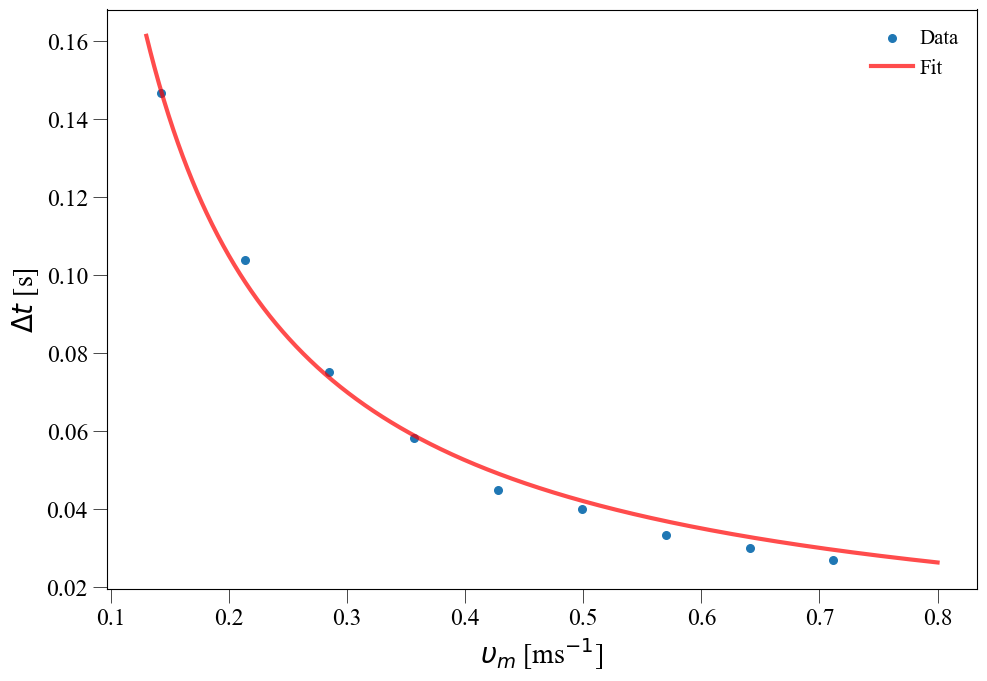
\includegraphics[scale=0.35]{t_v}
                \captionsetup{justification=centering, font=footnotesize}
                \captionof{figure}{Zavislost rychlosti magnetu $\upsilon_m$ na čase $\Delta t$.}
                \label{fig:t_v}
                \vspace{10pt}
                \raggedright
                \vspace{10pt}   
                \par \centering
                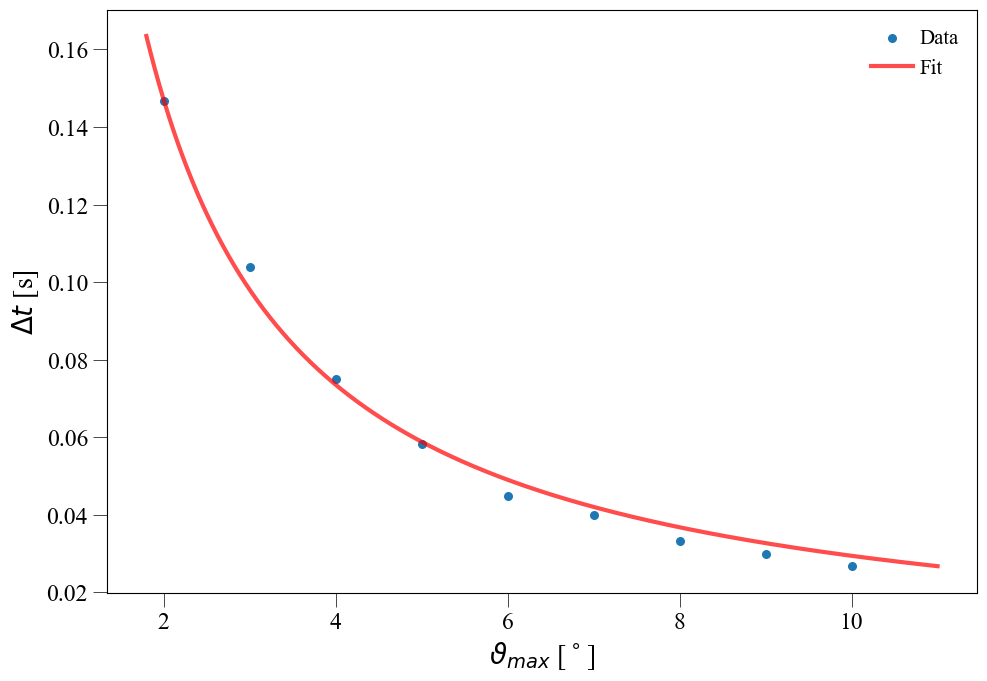
\includegraphics[scale=0.35]{t_u}
                \captionsetup{justification=centering, font=footnotesize}
                \captionof{figure}{Zavislost počátečního úhlu vychýlení magnetu $\vartheta_{max}$ na čase $\Delta t$.}
                \label{fig:t_u}
                \vspace{10pt}
                \raggedright
                Vynesli jsme také závislost amplitudy napěťových impulsů $U_{max}$ na počátečním úhlu vychýlení magnetu $\vartheta_{max}$. Graf je uveden na obrázku (5).
                \par Provedli jsme lineární aproximaci, ze které jsme získali hodnotu konstanty úměrnosti $k$:
                \begin{center}
                    $k$ = 0.127(2) $\frac{V}{^\circ}$
                \end{center}
    \end{minipage}
    \hspace{10pt}  
    \begin{minipage}[t]{0.5\textwidth} 
                \vspace{0pt}   
                \par \centering
                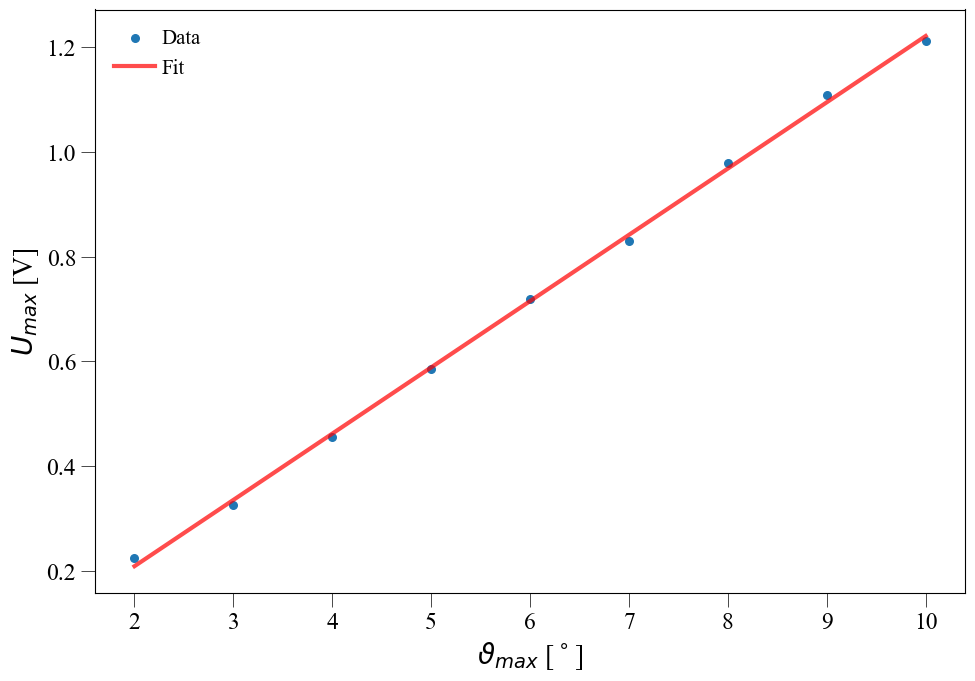
\includegraphics[scale=0.35]{u_u}
                \captionsetup{justification=centering, font=footnotesize}
                \captionof{figure}{Zavislost amplitudy napěťových impulsů $U_{max}$ na počátečním úhlu vychýlení magnetu $\vartheta_{max}$.}
                \label{fig:u_u}
                \vspace{10pt}
                \raggedright
                \par Odtud jsme podle vzorce (7) zjistili hodnotu magnetického dipólového momentu $m$:
                \begin{center}
                    $m$ = 1.34(7) Am$^2$
                \end{center}
                Tabulkové údaje pro výpočet:
                \begin{center}
                    $N$ = 1000
                    \vspace{5pt}
                    \par $\mu_0$ = 4$\pi$ $\cdot$ 10$^{-7}$ N m$^{-1}$
                \end{center}
            \subsection{Tlumení indukovaných pulzů}
                Pro analýzu tlumení kmitů analyzujeme závislost napětí indukovaného v cívce $U_M$ průchodem kyvadla přes ni na čase $t$. Za tímto účelem nastavíme různá napětí $R$, abychom si mohli představit míru tlumení kmitů. 
                \par Nejprve jsme analyzovali kmitání při odporech 1 M$\Omega$ a 1 k$\Omega$. Poté jsme vzali pouze maxima špiček a exponenciálně je aproximovali pomocí vzorce (8), čímž jsme získali koeficient $\beta$ pro každé z těchto napětí. Výsledky jsou uvedeny na obrázku (6).  
    \end{minipage}
\newpage
                \begin{figure}[ht!]
                    \centering
                    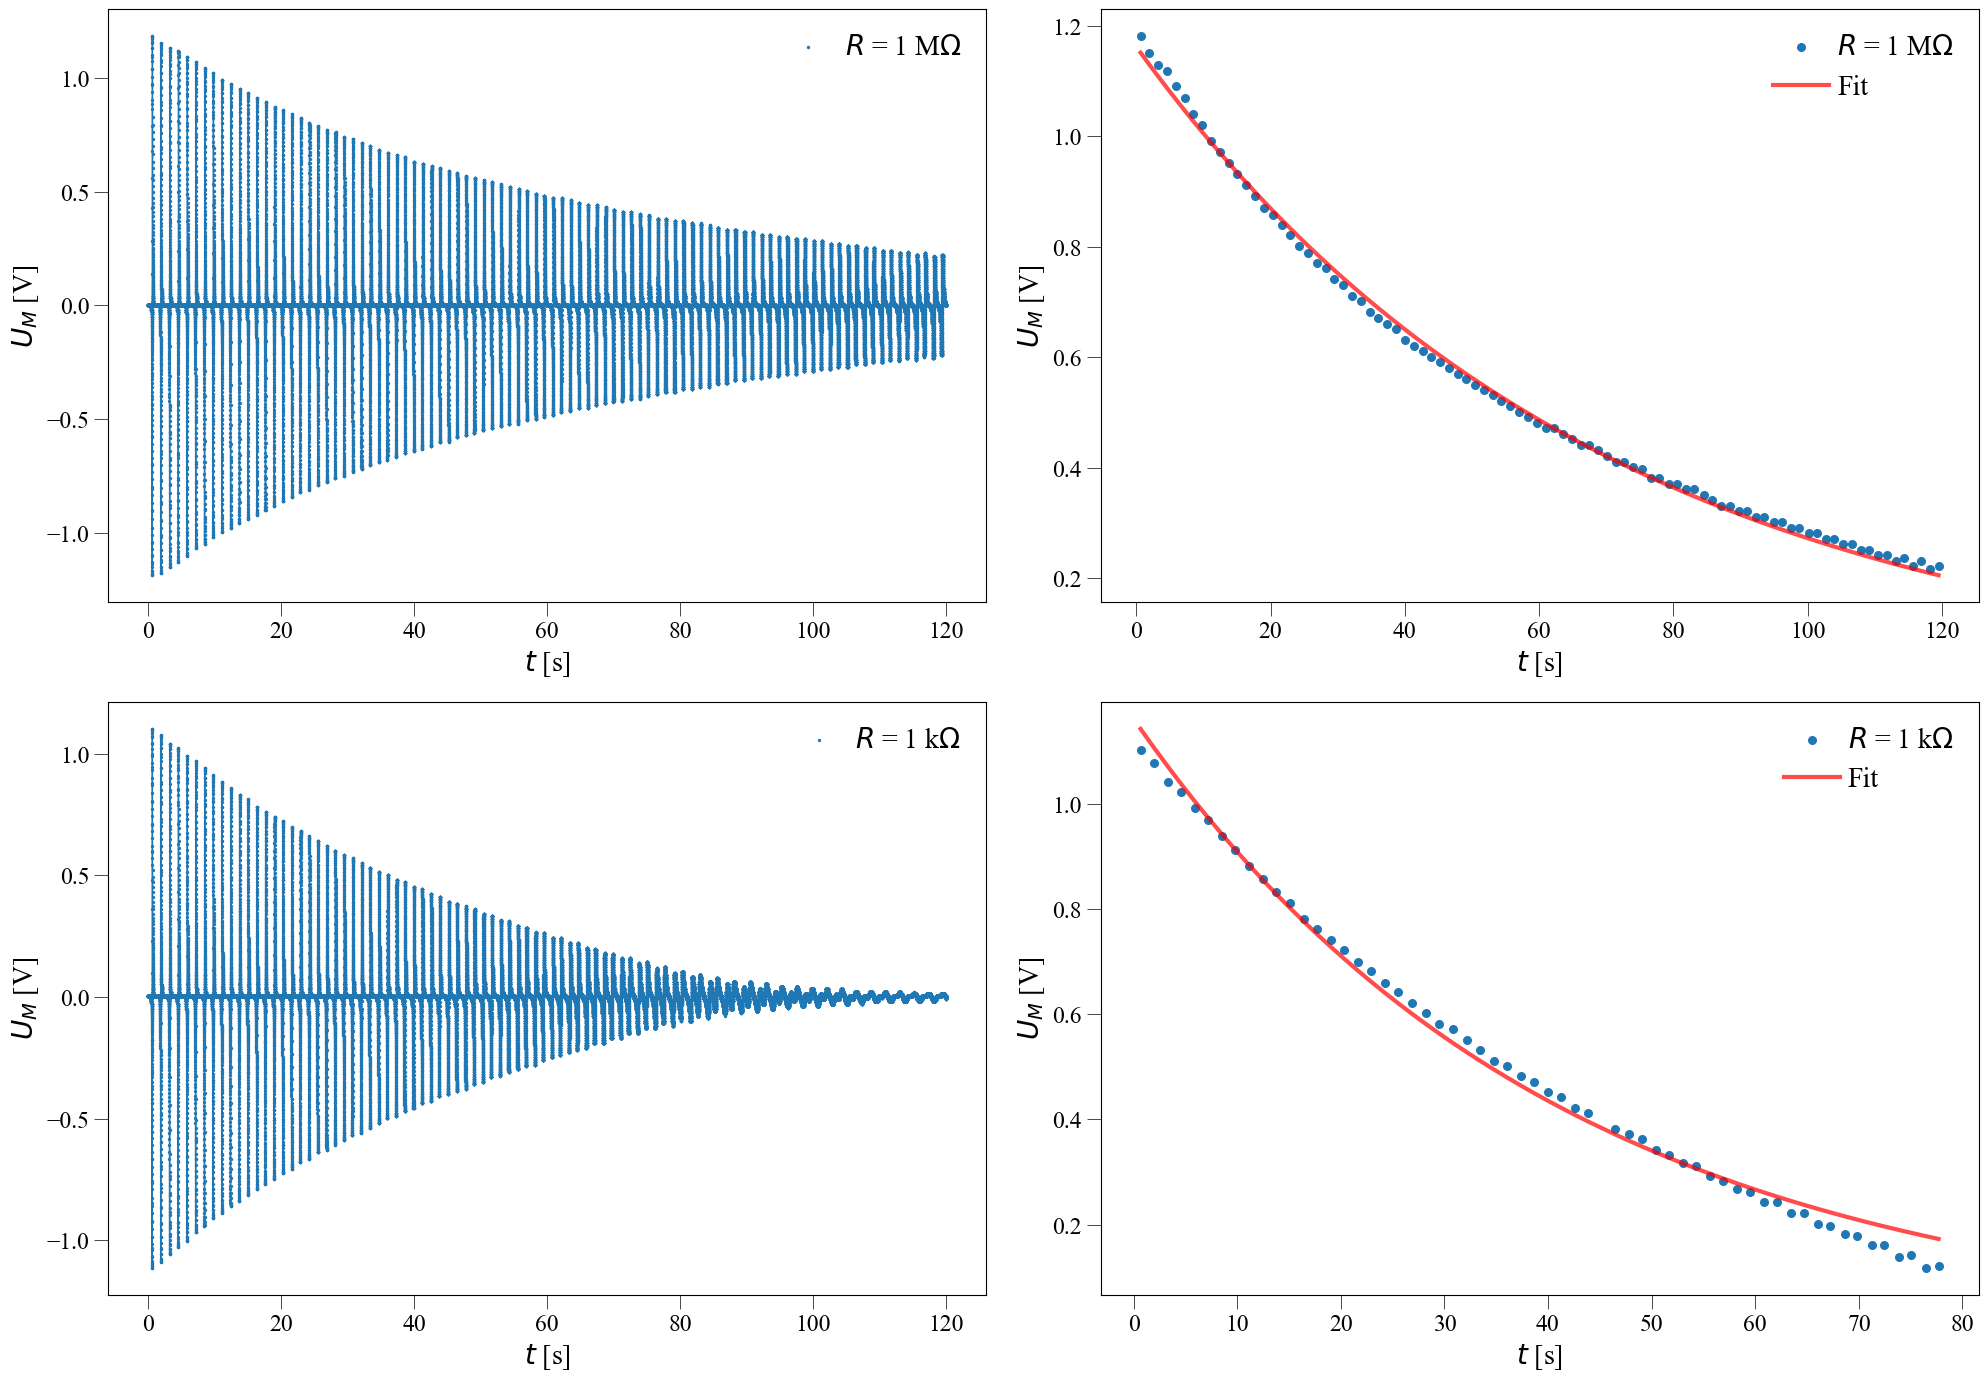
\includegraphics[scale=0.35]{beta_1}
                    \captionsetup{justification=centering, font=footnotesize}
                    \captionof{figure}{(vlevo nahoře) napětí při odporu $R$ = 1 M$\Omega$, (vpravo nahoře) maxima napětí při odporu $R$ = 1 M$\Omega$, (vlevo dole) napětí při odporu $R$ = 1 k$\Omega$, (vpravo dole) maxima napětí při odporu $R$ = 1 k$\Omega$.}
                    \label{fig:beta_1}
                \end{figure}
    \begin{minipage}[t]{0.5\textwidth} 
                Získali jsme tedy koeficienty $\beta_{1 M\Omega}$ a $\beta_{1 k\Omega}$ a napětí $U_{M,0}$ pro odpory 1 M$\Omega$ a 1 k$\Omega$:
                \begin{center}
                    \begin{multicols}{2}
                        $\beta_{1 M\Omega}$ = 0.01451(1) s$^{-1}$
                        \vspace{5pt}
                        \par $U_{M,1 M\Omega}$ = 1.163(4) V
                        \vspace{10pt}
                        \par $\beta_{1 k\Omega}$ = 0.0245(3) s$^{-1}$
                        \vspace{5pt}
                        \par $U_{M,1 k\Omega}$ = 1.161(9) V
                    \end{multicols}
                \end{center}
                Poté jsme změřili závislost maximálního pulzního napětí $U_M$ na čase $t$ pro odpory 20$\Omega$, 40$\Omega$, 60$\Omega$, 80$\Omega$, 100$\Omega$, 120$\Omega$, 150$\Omega$ a 200$\Omega$.
                \par Protože se jedná o relativně malý odpor, musíme vypočítat indukované napětí s ohledem na odpor cívky $R_C$. To lze provést podle následujícího vzorce:
                \begin{equation}
                    U_{M,ind} = \frac{R_C + R}{R} U_{M}
                \end{equation}
                kde $R$ je nastavený odpor.
                \par Poté jsme naměřené hodnoty zakreslili do grafu závislosti maximálních pulzů indukovaného napětí $U_{M,ind}$ na čase $t$, načež jsme pro každé z měření provedli lineární aproximaci podle vzorce (9). 
                \par Výsledky jsou uvedeny na obrázku (7).
                \par Tak jsme získali hodnoty koeficientu $\alpha$ pro každé z měření.
    \end{minipage}
    \hspace{10pt}
    \begin{minipage}[t]{0.5\textwidth} 
                Hodnoty koeficientu $\alpha$:
                \begin{center}
                    \begin{multicols}{2}
                        $\alpha_{20\Omega}$ = -0.154(3) s$^{-1}$
                        \par $\alpha_{40\Omega}$ = -0.112(2) s$^{-1}$
                        \par $\alpha_{60\Omega}$ = -0.081(1) s$^{-1}$
                        \par $\alpha_{80\Omega}$ = -0.072(1) s$^{-1}$
                        \par $\alpha_{100\Omega}$ = -0.063(1) s$^{-1}$
                        \par $\alpha_{120\Omega}$ = -0.0554(9) s$^{-1}$
                        \par $\alpha_{150\Omega}$ = -0.0496(7) s$^{-1}$
                        \par $\alpha_{200\Omega}$ = -0.0416(7) s$^{-1}$
                    \end{multicols}
                \end{center}
                \vspace{10pt}   
                \par \centering
                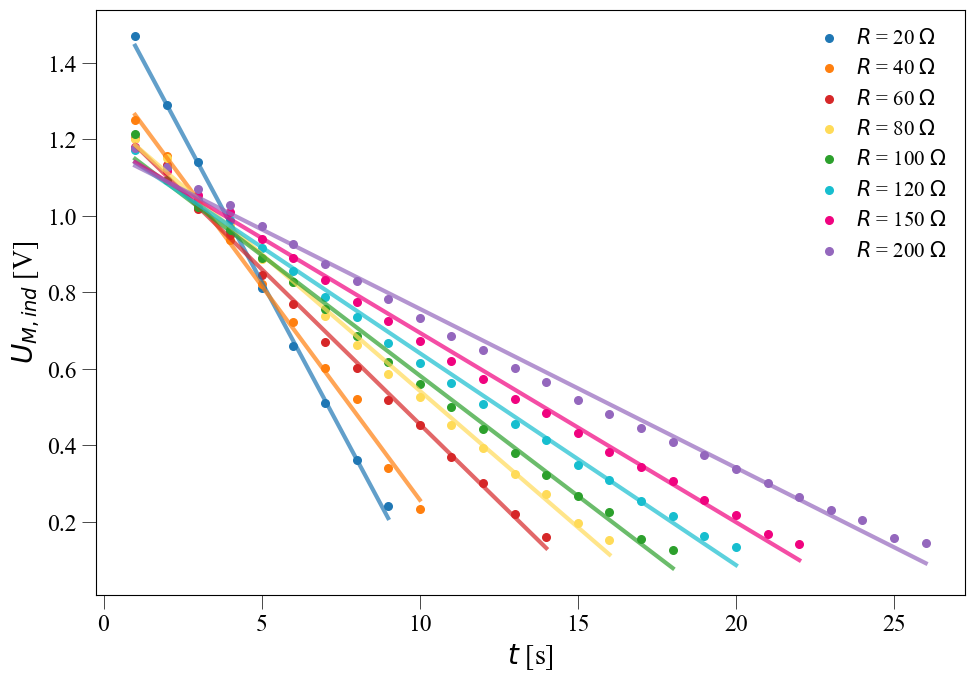
\includegraphics[scale=0.35]{alpha}
                \captionsetup{justification=centering, font=footnotesize}
                \captionof{figure}{Zavislost maximálních pulzů indukovaného napětí $U_{M,ind}$ na čase $t$ pro odpory 20$\Omega$, 40$\Omega$, 60$\Omega$, 80$\Omega$, 100$\Omega$, 120$\Omega$, 150$\Omega$ a 200$\Omega$.}
                \label{fig:alpha}
                \vspace{10pt}
                \raggedright
    \end{minipage}
\newpage
    \begin{minipage}[t]{0.5\textwidth} 
                Pro ověření linearity závislosti koeficientu $\alpha$ na odporu $R$ vykreslíme tyto hodnoty a lineárně je aproximujeme. Po aproximaci jsme získali následující hodnotu součinitele úměrnosti $A$:
                \begin{center}
                    $A$ = 0.097(6) $\frac{s}{V \Omega}$
                \end{center}
                Poté zkontrolujeme, kde přesně bude přímka procházet osou x. Výsledky jsou uvedeny na obrázku (8).
                Odtud vidíme, že přímka prochází osou x v bodě: 
                \vspace{10pt}   
                \par \centering
                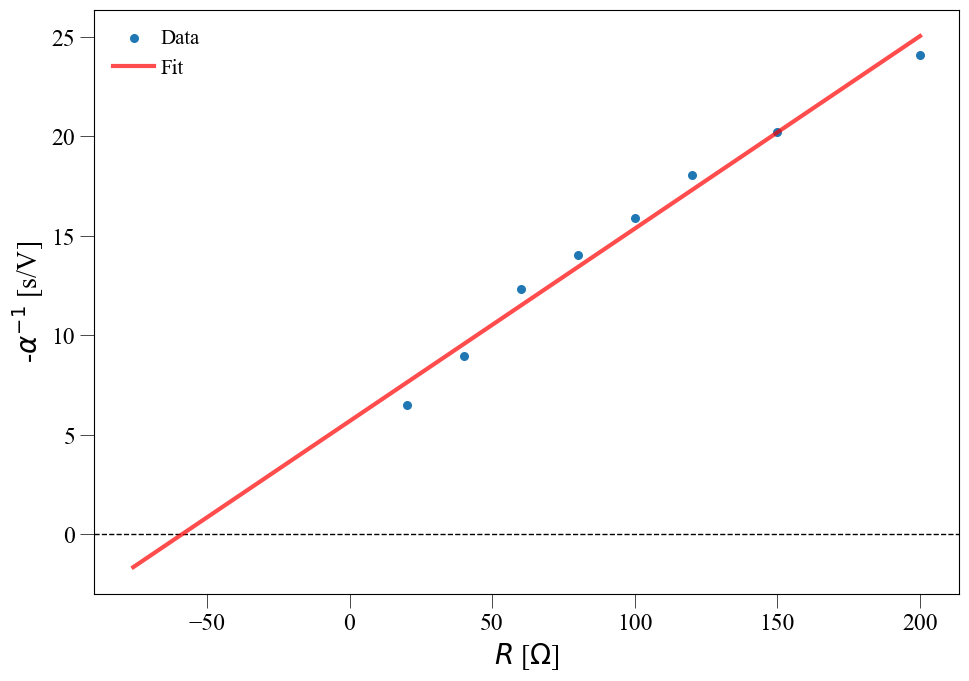
\includegraphics[scale=0.35]{alpha_2}
                \captionsetup{justification=centering, font=footnotesize}
                \captionof{figure}{Zavislost koeficientu $\alpha$ na odporu $R$.}
                \label{fig:alpha_2}
                \vspace{10pt}
                \raggedright
                \begin{center}
                    $R$ = -58.7 $\Omega$
                \end{center}
    \end{minipage}
    \hspace{10pt}
    \begin{minipage}[t]{0.5\textwidth} 
                K výpočtu veličin a jejich nejistot byla použita knihovna Uncertinties pro Python: \href{pypi.org/project/uncertainties}. Kód je přiložen k protokolu.
        \section{Závěr}  
            \subsection{Závislost indukovaných pulzů na výchylce, poloměr cívky a magnetický moment magnetu}
                Byl změřen poloměr cívky $a$ = 21(3) mm a magnetický dipólový moment $m$ = 1.34(7) Am$^2$.
                \par Dukazuje to, že $\Delta t$ je nepřímo úměrná $\upsilon_m$ a $\vartheta_{max}$.
            \subsection{Tlumení indukovaných pulzů}
                Byly změřeny koeficienty $\beta_{1 M\Omega}$ = 0.01451(1) s$^{-1}$ a $\beta_{1 k\Omega}$ = 0.0245(3) s$^{-1}$. Jejich rozdíl je způsoben elektromagnetickým tlumením. Hodnota součinitele úměrnosti $A$ = 0.097(6) $\frac{s}{V \Omega}$.
                \par Bylo zjištěno, že přímka prochází osou x v bodě $R$ = -58.7 $\Omega$. To ale muselo nastat při $R$ = 40 $\Omega$. Chyba je způsobena nepřesností měření koeficientu $\alpha$ pro dva poslední odporové hodnoty (150 $\Omega$ a 200 $\Omega$).
    \end{minipage}
    \vspace{30pt}
    \par K výpočtu chyb byl použit následující kód: 
    \begin{lstlisting}[language=Python, basicstyle=\tiny, breaklines=true, postbreak=\mbox{\textbackslashspace}]
        #Importing the libraries

        import matplotlib.pyplot as plt
        import numpy as np
        import pandas as pd
        from scipy import stats
        from scipy.optimize import curve_fit
        from uncertainties import *
        from uncertainties.umath import *

        #Reading data

        deg = pd.read_excel('data/deg.xlsx')

        MOhm_max = pd.read_csv('data/1MOhm.max', sep='\s+', header=None)
        kOhm_max = pd.read_csv('data/1kOhm.max', sep='\s+', header=None)
        MOhm = pd.read_csv('data/1MOhm.dat', sep='\s+', header=None)
        kOhm = pd.read_csv('data/1kOhm.dat', sep='\s+', header=None)

        Ohm_20 = pd.read_csv('data/20Ohm.max', sep='\s+', header=None)
        Ohm_40 = pd.read_csv('data/40Ohm.max', sep='\s+', header=None)
        Ohm_60 = pd.read_csv('data/60Ohm.max', sep='\s+', header=None)
        Ohm_80 = pd.read_csv('data/80Ohm.max', sep='\s+', header=None)
        Ohm_100 = pd.read_csv('data/100Ohm.max', sep='\s+', header=None)
        Ohm_120 = pd.read_csv('data/120Ohm.max', sep='\s+', header=None)
        Ohm_150 = pd.read_csv('data/150Ohm.max', sep='\s+', header=None)
        Ohm_200 = pd.read_csv('data/200Ohm.max', sep='\s+', header=None)

        # Constants and values

        L = 1.7 #m
        N = 1000 
        R_C = 40 #Ohm

        g = 9.80998 #m/s^2
        mu_0 = 4*np.pi*10**(-7) #N/A^2

        # Calculation 

        deg['dt'] = deg['t_max'] - deg['t_min']
        deg['U_max'] = (deg['U'] - deg['U_min'])/2
        deg['v_max'] = 2*np.sqrt(g*L)*np.sin(np.radians(deg['deg']/2))
        # print(deg)

        Ohm_20['U_ind'] = Ohm_20[2] * ((20+R_C)/(20))
        Ohm_40['U_ind'] = Ohm_40[2] * ((40+R_C)/(40))
        Ohm_60['U_ind'] = Ohm_60[2] * ((60+R_C)/(60))
        Ohm_80['U_ind'] = Ohm_80[2] * ((80+R_C)/(80))
        Ohm_100['U_ind'] = Ohm_100[2] * ((100+R_C)/(100))
        Ohm_120['U_ind'] = Ohm_120[2] * ((120+R_C)/(120))
        Ohm_150['U_ind'] = Ohm_150[2] * ((150+R_C)/(150))
        Ohm_200['U_ind'] = Ohm_200[2] * ((200+R_C)/(200))

        # Define the polynomial function

        def polynomial_fit(values, A):
            return A/values

        # Use curve_fit to find the parameters A
        initial_guess = [0.02]  # Initial guess for parameters A
        params, covariance = curve_fit(polynomial_fit, deg['v_max'], deg['dt'], p0=initial_guess)

        # Extract the optimized parameters
        a_optimized = params
        a_error = np.sqrt(np.diag(covariance))

        a_comb = ufloat(a_optimized, a_error)

        # Print the optimized parameters
        print('a =', a_comb*10**(3), 'mm')

        #Best-fit line

        v_val = np.linspace(0.13, 0.8, 1000)

        v_fit = polynomial_fit(v_val , a_optimized)

        # Define the polynomial function

        def polynomial_fit(values, A):
            return A/values

        # Use curve_fit to find the parameters A
        initial_guess = [0.02]  # Initial guess for parameters A
        params, covariance = curve_fit(polynomial_fit, deg['deg'], deg['dt'], p0=initial_guess)

        # Extract the optimized parameters
        A_optimized = params
        A_error = np.sqrt(np.diag(covariance))

        A_comb = ufloat(A_optimized, A_error)

        # Print the optimized parameters
        print('A =', A_comb*10**(3), 'deg s')

        #Best-fit line

        deg_val = np.linspace(1.8, 11, 1000)

        deg_fit = polynomial_fit(deg_val , A_optimized)


        #Calculate linear regression

        slope, intercept, r_value, p_value, std_err = stats.linregress(deg['deg'], deg['U_max'])
        k = ufloat(slope, std_err)

        print(f'k =', k, 'V/deg')

        #Best fit line 
        u_fit = slope * np.array(deg['deg']) + intercept

        m = ((25*np.sqrt(5))/24) * ((k*a_comb**2)/(N*mu_0*np.sqrt(g*L))) * ufloat(53.2,2.3)

        print(f'm =', m, 'Am^2')

        # Define the polynomial function

        def polynomial_fit(values, A, B):
            return A * np.exp(-B * values)

        # Use curve_fit to find the parameters A and B
        initial_guess = [1.5, 0.02]  # Initial guess for parameters A and B
        params, covariance = curve_fit(polynomial_fit, MOhm_max[1], MOhm_max[2], p0=initial_guess)

        # Extract the optimized parameters
        A_optimized, B_optimized = params
        A_error, B_error = np.sqrt(np.diag(covariance))

        U_M_0 = ufloat(A_optimized, A_error)
        beta_M_ohm = ufloat(B_optimized, B_error)

        # Print the optimized parameters
        print('U_M_0 =', U_M_0, 'V')
        print('beta_M_ohm =', beta_M_ohm, 's^-1')

        #Best-fit line

        MOhm_fit = polynomial_fit(MOhm_max[1], A_optimized, B_optimized)

        # Define the polynomial function

        def polynomial_fit(values, A, B):
            return A * np.exp(-B * values)

        # Use curve_fit to find the parameters A and B
        initial_guess = [1.5, 0.02]  # Initial guess for parameters A and B
        params, covariance = curve_fit(polynomial_fit, kOhm_max[1], kOhm_max[2], p0=initial_guess)

        # Extract the optimized parameters
        A_optimized, B_optimized = params
        A_error, B_error = np.sqrt(np.diag(covariance))

        U_M_0 = ufloat(A_optimized, A_error)
        beta_k_ohm = ufloat(B_optimized, B_error)

        # Print the optimized parameters
        print('U_M_0 =', U_M_0, 'V')
        print('beta_k_ohm =', beta_k_ohm, 's^-1')

        #Best-fit line

        kOhm_fit = polynomial_fit(kOhm_max[1], A_optimized, B_optimized)

        #Calculate linear regression

        slope, intercept, r_value, p_value, std_err = stats.linregress(Ohm_20[0], Ohm_20['U_ind'])
        alpha_20 = ufloat(slope, std_err)
        print(f'alpha_20 =', alpha_20, 'V/s')
        alpha_20_fit = slope * np.array(Ohm_20[0]) + intercept

        slope, intercept, r_value, p_value, std_err = stats.linregress(Ohm_40[0], Ohm_40['U_ind'])
        alpha_40 = ufloat(slope, std_err)
        print(f'alpha_40 =', alpha_40, 'V/s')
        alpha_40_fit = slope * np.array(Ohm_40[0]) + intercept

        slope, intercept, r_value, p_value, std_err = stats.linregress(Ohm_60[0], Ohm_60['U_ind'])
        alpha_60 = ufloat(slope, std_err)
        print(f'alpha_60 =', alpha_60, 'V/s')
        alpha_60_fit = slope * np.array(Ohm_60[0]) + intercept

        slope, intercept, r_value, p_value, std_err = stats.linregress(Ohm_80[0], Ohm_80['U_ind'])
        alpha_80 = ufloat(slope, std_err)
        print(f'alpha_80 =', alpha_80, 'V/s')
        alpha_80_fit = slope * np.array(Ohm_80[0]) + intercept

        slope, intercept, r_value, p_value, std_err = stats.linregress(Ohm_100[0], Ohm_100['U_ind'])
        alpha_100 = ufloat(slope, std_err)
        print(f'alpha_100 =', alpha_100, 'V/s')
        alpha_100_fit = slope * np.array(Ohm_100[0]) + intercept

        slope, intercept, r_value, p_value, std_err = stats.linregress(Ohm_120[0], Ohm_120['U_ind'])
        alpha_120 = ufloat(slope, std_err)
        print(f'alpha_120 =', alpha_120, 'V/s')
        alpha_120_fit = slope * np.array(Ohm_120[0]) + intercept

        slope, intercept, r_value, p_value, std_err = stats.linregress(Ohm_150[0], Ohm_150['U_ind'])
        alpha_150 = ufloat(slope, std_err)
        print(f'alpha_150 =', alpha_150, 'V/s')
        alpha_150_fit = slope * np.array(Ohm_150[0]) + intercept

        slope, intercept, r_value, p_value, std_err = stats.linregress(Ohm_200[0], Ohm_200['U_ind'])
        alpha_200 = ufloat(slope, std_err)
        print(f'alpha_200 =', alpha_200, 'V/s')
        alpha_200_fit = slope * np.array(Ohm_200[0]) + intercept

        alpha_list = [-alpha_20.nominal_value**(-1), -alpha_40.nominal_value**(-1), -alpha_60.nominal_value**(-1), -alpha_80.nominal_value**(-1), -alpha_100.nominal_value**(-1), -alpha_120.nominal_value**(-1), -alpha_150.nominal_value**(-1), -alpha_200.nominal_value**(-1)]
        R_list = [20, 40, 60, 80, 100, 120, 150, 200]

        slope, intercept, r_value, p_value, std_err = stats.linregress(R_list, alpha_list)
        A = ufloat(slope, std_err)
        print(f'A =', A, 'V/s')

        R_values = np.linspace(-75.8, 200, 1000)

        A_fit = slope * R_values + intercept
    \end{lstlisting}
\end{document}